% UTF-8 encoding
\begin{savequote}[75mm]
Nulla facilisi. In vel sem. Morbi id urna in diam dignissim feugiat. Proin molestie tortor eu velit. Aliquam erat volutpat. Nullam ultrices, diam tempus vulputate egestas, eros pede varius leo.
\qauthor{Quoteauthor Lastname}
\end{savequote}

\chapter{The first chapter}

\newthought{There's \zh{新浪微博} something to be said} for having a good opening line. Morbi commodo, ipsum sed pharetra gravida, orci  $x = 1/\alpha$ magna rhoncus neque, id pulvinar odio lorem non turpis \cite{Guichard2013}. Nullam sit amet enim. Suspendisse id velit vitae ligula volutpat \zh{新浪微博} condimentum. Aliquam erat volutpat. Sed quis velit. Nulla facilisi. Nulla libero. Vivamus pharetra posuere sapien. Nam consectetuer. Sed aliquam, nunc eget euismod ullamcorper, \zh{新浪微博}lectus nunc ullamcorper orci, fermentum bibendum enim nibh eget ipsum. Donec porttitor ligula eu dolor. Maecenas vitae nulla consequat libero cursus venenatis. Nam magna enim, accumsan eu, blandit sed, blandit a, eros.

\zh{}
\zh{新浪微博}


\begin{figure}[h]
    \centering
    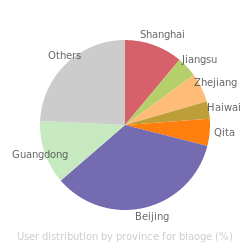
\includegraphics{figures/memes/geo_pie_biaoge_Aug_20_2012_Sep_02_2012.png}
    \caption[Short version for LoF]{Long version to appear next to the figure}
    \label{fig:geopie_biaoge}
\end{figure}

La figure~\ref{fig:geopie_biaoge} montre une photographie de toucan.

\begin{figure}[htp]
    \centering
    \subfloat[Légende 1]{\label{fig:edge-a}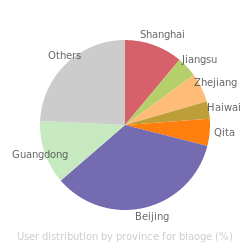
\includegraphics[scale=0.5]{figures/memes/geo_pie_biaoge_Aug_20_2012_Sep_02_2012.png}}
    \hspace{5pt}

    \subfloat[Légende 2]{\label{fig:edge-a}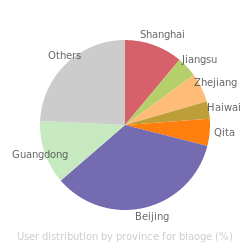
\includegraphics[scale=0.5]{figures/memes/geo_pie_biaoge_Aug_20_2012_Sep_02_2012.png}}
    \hspace{5pt}

    \subfloat[Légende 3]{\label{fig:edge-a}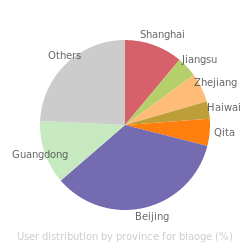
\includegraphics[scale=0.5]{figures/memes/geo_pie_biaoge_Aug_20_2012_Sep_02_2012.png}}
    \hspace{5pt}
    \caption{Différents algorithmes de détection des contours}
    \label{fig:multiple}
\end{figure}